\subsection{Materiais e bases de dados}
\label{subsec:ml-dataset}

Esta parte do método trata do modelo de detecção. Ela parte do RSSI, o
metadado de recepção definido na Seção~\ref{subsec:camada_fisica_lora}, e
entrega o detector que o \textit{gateway} da Seção~\ref{sec:requisitos_infra}
executa, descrito na Seção~\ref{subsec:ml-protocolo-borda}. O modelo é estimado
com o \textit{dataset} Tour Perret,
publicado pelo CampusIoT da Université Grenoble Alpes \cite{tourperret_dataset}.
Ele reúne os eventos de cinco nós sensores instalados na Tour Perret, em
Grenoble, recebidos de 25/06/2021 a 23/06/2023 por um servidor de rede
ChirpStack v3, num total de 421.937 mensagens. O arquivo usado é o oficial,
conferido pelo resumo SHA-256 publicado com ele. Cada evento de
\textit{uplink} traz uma lista com uma entrada por \textit{gateway} que recebeu
o quadro, com o RSSI medido naquele \textit{gateway} \cite{brocaarintegration}.

O \textit{dataset} vem de sensores em operação real e não tem rótulos de ataque.
Por isso ele serve para aprender o comportamento esperado do RSSI, e a
capacidade de detecção é medida com desvios sintéticos, como descrito na
Seção~\ref{subsec:ml-protocolo-deteccao}.

\subsection{Limpeza e recorte da série}
\label{subsec:ml-limpeza}
% sec:selecao_variaveis: rótulo citado pelas Seções 2.1 e 3.1 (barea); aqui se define que o modelo usa só o RSSI.
\label{sec:selecao_variaveis}

A limpeza segue regras numeradas, cada uma com a contagem de linhas depois de
aplicada, como mostram a Tabela~\ref{tab:ml-limpeza} e a
Figura~\ref{fig:ml-funil}. Os dados ficam em duas tabelas, uma de quadros e
outra de recepções, segundo o princípio de uma linha por observação
\cite{wickham2014tidy}. As regras têm quatro papéis diferentes. L1 e L4 removem
registros que não são medidas novas. L2 e L3 só organizam os dados. L6 e L8 não
removem dados inválidos. Elas fazem o recorte do estudo, escolhendo um nó
sensor e um trecho contínuo. L7 e L9 apenas marcam quadros, sem remover nada, e
L5 registra a decisão de não filtrar o RSSI.

\begin{table}[htb]
	\centering
	\caption{Regras de limpeza e recorte da série de RSSI}
	\label{tab:ml-limpeza}
	\begin{tabular}{llr}
		\hline
		\textbf{Regra} & \textbf{O que faz} & \textbf{Linhas depois} \\
		\hline
		L1 & Mantém só eventos de \textit{uplink} & 421.906 \\
		L2 & Usa o instante de arquivamento como eixo de tempo & 421.906 \\
		L3 & Separa quadros e recepções (recepções) & 3.559.119 \\
		L4 & Remove retransmissões (quadros) & 398.699 \\
		L5 & Não aplica limite físico ao RSSI & 398.699 \\
		L6 & Seleciona o nó sensor \texttt{441a1ed9} & 193.442 \\
		L7 & Marca trocas de taxa de dados e quedas do FCnt & 193.442 \\
		L8 & Seleciona o maior trecho sem lacuna maior que 1~h & 58.540 \\
		L9 & Marca os quadros sem RSSI no \textit{gateway} escolhido & 58.540 \\
		\hline
	\end{tabular}
	\legend{Fonte: elaborado pelos autores.}
\end{table}

\begin{figure}[htb]
	\centering
	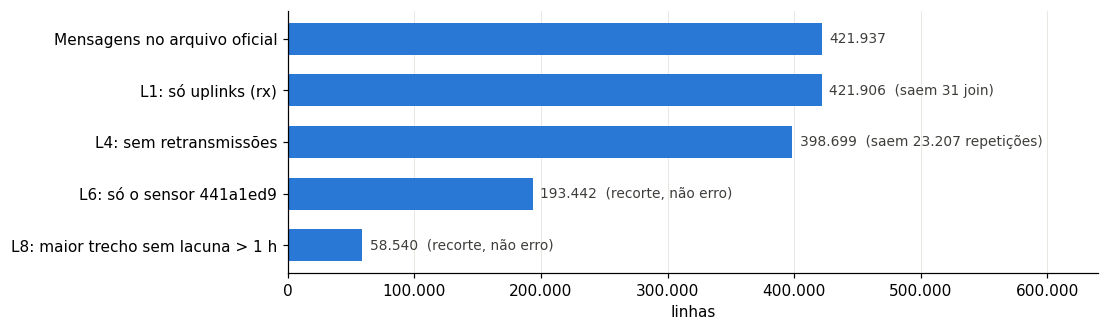
\includegraphics[width=0.85\textwidth]{tadaki/figuras/ml-funil-limpeza.png}
	\caption{Quantidade de linhas depois de cada etapa da limpeza e do recorte}
	\label{fig:ml-funil}
	\legend{Fonte: elaborado pelos autores.}
\end{figure}

A regra L4 trata como retransmissão o quadro do mesmo nó sensor com o mesmo
FCnt do anterior, recebido em menos de 60~s, porque o FCnt não sobe quando o
mesmo quadro é reenviado \cite{lorawan103}. No trecho usado, a janela de 60~s
não muda nada, pois de 10~s a sem limite são sempre as mesmas 4
retransmissões. A regra L5 deixa o RSSI sem filtro, porque no trecho usado ele
fica entre $-120$ e $-90$~dBm e um valor extremo pode trazer informação sobre o
processo \cite{hyndman2021}, que é justamente o que a detecção procura.

O estudo usa só o RSSI, de um nó sensor e de um \textit{gateway}. Entre os cinco
nós sensores, o \texttt{441a1ed9} tem ao mesmo tempo o maior número de quadros
(193.442), a taxa de dados mais estável (99,99\% em DR5, com 13 trocas) e o
maior trecho contínuo (58.540 quadros, contra no máximo 24.992 dos outros). O
\textit{gateway} \texttt{17459c66} é o de maior cobertura desse nó sensor, com
97,2\% dos quadros. O maior trecho sem intervalo acima de 3.600~s vai de
16/11/2021 a 08/06/2022, em 203,7 dias, e é o mesmo para qualquer limite entre
3.600 e 14.400~s.

\subsection{Preparação da série}
\label{subsec:ml-preparacao}

Depois da limpeza, quatro decisões transformam os quadros em uma série pronta
para o modelo. A série começa no primeiro quadro com RSSI observado, porque
antes dele não há valor anterior a repetir, o que descarta 4 quadros e deixa
58.536. O quadro que o \textit{gateway} escolhido não recebeu, 2,8\% do
trecho, recebe o último valor observado e fica marcado. Essa forma de
preencher usa só o passado. Uma alternativa medida, deixar o vazio para o
próprio modelo tratar, mudou o RMSE de validação do ARIMA por canal de
1,136 para 1,135~dBm.

O eixo da série é a ordem dos quadros, e não o relógio, porque o modelo supõe
passos iguais. O nó sensor transmite a intervalos regulares. O intervalo entre
quadros consecutivos tem mediana de 300,0~s e fica até 300,03~s em 99\% dos
casos, e só 24 dos 58.535 intervalos passam de 600~s. A divisão é cronológica,
como mostra a Tabela~\ref{tab:ml-divisao}.

\begin{table}[htb]
	\centering
	\caption{Divisão da série em treino, validação e teste}
	\label{tab:ml-divisao}
	\begin{tabular}{lrlr}
		\hline
		\textbf{Parte} & \textbf{Quadros} & \textbf{Período (UTC)} & \textbf{Sem RSSI} \\
		\hline
		Treino (70\%) & 40.975 & 16/11/2021 a 08/04/2022 & 1.355 \\
		Validação (15\%) & 8.780 & 08/04/2022 a 08/05/2022 & 121 \\
		Teste (15\%) & 8.781 & 08/05/2022 a 08/06/2022 & 138 \\
		\hline
	\end{tabular}
	\legend{Fonte: elaborado pelos autores.}
\end{table}

O treino estima os coeficientes do modelo. A validação serve a todas as
escolhas, a ordem do modelo e o limiar do alarme. O teste é usado uma única vez
para cada configuração final.

\subsection{Protocolo de avaliação da previsão}
\label{subsec:ml-protocolo}

Toda previsão é um passo à frente. Os coeficientes do ARIMA são estimados uma
vez no treino e depois aplicados, fixos, ao resto da série
\cite{statsmodelsapply}, de modo que cada quadro é previsto com os valores
reais até o quadro anterior, como faria o \textit{gateway}. A diferenciação é
decidida pelo teste KPSS no treino, a ordem é escolhida pelo RMSE na validação,
e cada configuração final é avaliada uma única vez no teste.

O erro é medido pelo RMSE e pelo MAE da Seção~\ref{subsec:ml-avaliacao} e
também pela mediana do erro absoluto, que indica o erro típico de um quadro.
As três medidas usam só os quadros com RSSI observado, porque num quadro
preenchido o \textit{random walk} acerta por construção.

O modelo é comparado com duas referências. A primeira é o \textit{random walk}
da Equação~\ref{eq:ml-random-walk}. A segunda, mais exigente, é o
\textit{random walk} por canal, que repete o último valor observado no mesmo
canal de frequência. Ganhar desta segunda referência mostra que o modelo
acrescenta algo além de separar os canais.

A robustez dos resultados é verificada de quatro formas. O mesmo procedimento é
repetido no \textit{gateway} \texttt{100210b9}. A ordem do modelo é variada um
parâmetro de cada vez, para ver se o resultado depende de uma ordem
específica. A execução completa, do \textit{dataset} bruto aos resultados, é
refeita numa cópia isolada do projeto. Por fim, para medir quanto dado de
treino basta, o ARIMA é estimado com treinos de 6~h a 142 dias, todos
terminando no fim do treino e avaliados na mesma validação. Um tamanho basta
quando o RMSE fica abaixo do \textit{random walk} por canal e no máximo 20\%
acima do obtido com o treino inteiro.

\subsection{Protocolo da detecção}
\label{subsec:ml-protocolo-deteccao}

A detecção usa a regra da Equação~\ref{eq:ml-deteccao} sobre o erro do modelo
final. Em cada canal, o limiar $\tau$ é o quantil de 99\% do erro absoluto na
validação, o que fixa cerca de 1\% de alarmes falsos sem depender da suposição
de normalidade \cite{hundman2018spacecraft}. O limiar nunca fica abaixo de
1,5~dB, porque o \textit{gateway} informa o RSSI em valores inteiros de dB.

Como o \textit{dataset} não tem ataques identificados, a detecção é medida com
desvios sintéticos, somados a uma cópia do teste. Cada desvio é um degrau de
$+\Delta$ ou $-\Delta$~dB, com $\Delta$ de 1 a 10~dB, em dois formatos, um de 12
quadros, cerca de 1~h, e outro de um só quadro. O sentido positivo segue o
efeito do \textit{jamming} reativo sobre o RSSI \cite{ruotsalainen2022jamming}.
Cada combinação é aplicada em 300 posições sorteadas do teste, uma de cada vez,
com semente fixa, e o valor alterado entra no histórico do modelo, como
aconteceria na borda. As medidas são a taxa de alarmes falsos no teste sem
desvio e a fração dos desvios com ao menos um alarme, com intervalo de
confiança de 95\% pelo método de Wilson.

Para saber quanto da detecção vem do modelo, o mesmo protocolo é aplicado a um
detector mais simples, que usa como previsão o \textit{random walk} por canal.
Como o RSSI é inteiro, o erro desse detector também é inteiro, e o limiar por
quantil não consegue fixar o alarme falso em 1\%. Por isso ele é avaliado em
duas versões. A primeira usa a mesma regra, o que dá menos alarmes falsos que o
ARIMA, e a segunda usa o limiar um valor inteiro abaixo, o que dá mais.

\subsection{Execução do detector no microcontrolador}
\label{subsec:ml-protocolo-borda}

Com os coeficientes fixos, a previsão um passo à frente do ARIMA$(0,1,1)$ é a
suavização exponencial simples \cite{hyndman2021}, como na
Equação~\ref{eq:ml-borda}, em que $\alpha = 1 + \theta$ e $\theta$ é o
coeficiente de média móvel estimado no treino de cada canal.
\begin{equation}
	\hat{y}_{t+1} = \hat{y}_t + \alpha \left( y_t - \hat{y}_t \right)
	\label{eq:ml-borda}
\end{equation}

Por isso o detector não precisa de biblioteca de séries temporais. Para cada
canal ele guarda $\alpha$, o limiar e a última previsão. Esses valores são
exportados do Python para um arquivo de cabeçalho em C++, e o mesmo código é
compilado para o computador e para a placa Heltec WiFi LoRa 32 V3, com ESP32-S3,
usada pela frente de infraestrutura. A conferência compara, quadro a quadro,
a previsão e o alarme do detector com os do Python, na série de teste e na mesma
série com um desvio sintético de $+5$~dB por 12 quadros. No \textit{gateway} do
protótipo, o detector roda depois do registro de cada quadro autenticado, sem
alterar o dado registrado, e um botão da placa soma um desvio sintético ao RSSI
que o detector recebe, para simular um ataque.

